\chapter{Tecnologie di sviluppo del back-end}
\label{chap:tecnologie di sviluppo del back-end}

L’architettura scelta per OVL Dashboard segue il modello client-server, in cui il client rappresenta l’interfaccia, mentre il server svolge il compito di implementazione delle logiche applicative e di conservazione dei dati. La comunicazione tra le due componenti avviene tramite Internet, in modo tale da permettere a qualunque utente della piattaforma di raggiungerla facilmente dal dispositivo e dal luogo che preferisce.

Il back-end di OVL Dashboard è composto, come visto in precedenza, da diversi elementi: il server di storage, il server di autenticazione, un database MySQL per la memorizzazione delle connessioni e un secondo database noSQL per la gestione degli utenti. Tutti questi apparati sono mantenuti all'interno del cloud computing di AWS (Amazon Web Services)\footnote{AWS: \url{https://aws.amazon.com}}.

Il server di storage offre gli endpoint necessari a soddisfare i vari casi d'uso provenienti dal front-end, cioè dalla dashboard. Esso permette l'effettiva gestione delle connessioni della rete virtuale mediante la comunicazione con il database MySQL (condiviso e gestito con Guacamole).

Il server di autorizzazione, invece, rende possibile l'accesso a tutti i servizi di OpenVirtualLab con l'utilizzo di un singolo account. Questo server è implementato partendo da un fork del progetto OpenID Connect, che consente ai client di tutti i tipi, inclusi client Web, mobili e JavaScript, di richiedere e ricevere informazioni su sessioni autenticate e utenti finali. L'adozione di un server di autenticazione permette di mantenere separati la logica di gestione degli account e le funzionalità legate ad essi dai servizi OVL dell'azienda Themis s.r.l. Per la memorizzazione delle informazioni relative agli account è stato utilizzato MongoDB, un database documentale che offre alte prestazioni.

\section{AWS}
\label{sec:AWS}

Con il termine “cloud computing” si indicano una serie di tecnologie che permettono di elaborare, archiviare e memorizzare dati grazie all'utilizzo di risorse hardware e software distribuite nella rete.
L’innovazione apportata dalle configurazioni cloud riguarda la distribuzione in rete dei servizi, la semplice scalabilità dell'infrastruttura, le maggiori affidabilità e continuità del servizio e l’erogazione in tempi molto rapidi di nuove risorse di calcolo e memorizzazione.
Con servizi cloud si intendono server pilotati da un software che ne mette a disposizione le capacità di calcolo (CPU) e di memorizzazione (dischi); i servizi forniti vengono dislocati automaticamente tra tutti i server disponibili e in caso di necessità nuovi server possono essere facilmente aggiunti per aumentare la capacità complessiva del sistema. In particolare, AWS è una piattaforma di servizi cloud sicura in grado di offrire potenza di elaborazione, storage di database, distribuzione dei contenuti e altre funzionalità a supporto del dimensionamento e della crescita delle attività aziendali.
Il servizio per eccellenza di AWS è rappresentato da EC2, Elastic Computing Cloud. Esso è un servizio di AWS che fornisce un’infrastruttura web per disporre di macchine virtuali completamente on demand. Tramite EC2 è possibile configurare, avviare, spegnere e clonare istanze di macchine virtuali costruite totalmente secondo le proprie necessità. Per quanto riguarda i servizi di database abbiamo usato RDS (Amazon Relational Database Service), che è un servizio che semplifica configurazione, utilizzo e ridimensionamento di database relazionali nel cloud. Offre capacità ridimensionabili ad un costo vantaggioso e gestisce al contempo lunghe attività amministrative del database, in modo da consentire all'utente di concentrarsi sulle proprie applicazioni e sul proprio business. Amazon RDS permette di scegliere tra sei motori di database comuni: Amazon Aurora, PostgreSQL, MySQL, MariaDB, Oracle e Microsoft SQL Server. I due servizi appena descritti sono stati quelli di maggior interesse per lo sviluppo della dashboard.

\section{Node.js e Express}
\label{sec:Node.js e express}

Per lo sviluppo dei entrambi i server è stato adottato Node.js, un’applicazione, per la precisione un framework, nata nel 2009, che viene usata per scrivere applicazioni in Javascript lato server.
Il codice su Node.js, infatti, viene fatto girare da V8. Sto parlando del motore JavaScript open source di Google, scritto in C++ e utilizzato in Google Chrome. Si tratta di una soluzione lato server basata su un modello di I/O asincrono che opera sugli eventi. Node richiede al sistema operativo di ricevere notifiche al verificarsi di determinati eventi, e rimane quindi in attesa fino alla notifica stessa: solo in tale momento torna attivo per eseguire le istruzioni previste in una funzione di callback, così chiamata perché da eseguire una volta ricevuta la notifica che il risultato dell'elaborazione del sistema operativo è disponibile.
Nonostante un singolo processo Node.js venga sempre eseguito su un singolo thread, sui sistemi multicore è possibile creare un cluster. Per fare ciò l’applicazione Node.js crea un insieme di processi figli detti worker e suddivide le connessioni in entrata in modo equo tra di essi.
In gran parte dei server web, le operazioni di I/O sono bloccanti: il thread del server viene infatti bloccato dal sistema operativo per il tempo necessario alla conclusione dell’operazione. Questo problema è stato risolto rendendo i web server multi-threaded, e creando un thread per ogni connessione. La creazione e la gestione di thread però non è sempre efficiente, soprattutto in caso si grandi quantità di connessioni. Node.js invece utilizza un modello orientato agli eventi, e questo gli consente di compiere le operazioni di I/O in modo non bloccante nonostante venga eseguito su un singolo thread. Ogni operazioni di I/O è infatti asincrona: l’operazione viene fatta partire, ed è necessario registrare una funzione di callback che verrà richiamata da Node.js appena l’operazione sarà terminata. Questa caratteristica lo rende particolarmente efficiente per le applicazioni web, in cui le operazioni di rete sono frequenti e di vitale importanza.

Insieme a Node.js è stato utilizzato Express, un web framework minimale e flessibile, che offre strumenti di base per creare più velocemente applicazioni in Node.
Express mette a disposizione dei Routers, sulle quali posso definire le mie rotte, i miei endpoint dei servizi. La loro struttura è molto semplice. Occorre specificare per ogni endpoint il metodo di richiesta http, il path della route e la funzione handler da eseguire al match della route.  

La scelta di Node.js ha sicuramente accelerato lo sviluppo. L’utilizzo di un linguaggio di programmazione comune sia dal lato client che dal lato server ha consentito alla parte di team che si occupa del front-end di revisionare, eseguire il debug e in alcuni casi contribuire alla parte back-end dell'applicazione senza la necessità di dover apprendere un altro linguaggio di programmazione. Lavorare con Express poi semplifica notevolmente la realizzazione di applicazioni web, che grazie a Router permette di strutturare bene le risorse.

\section{Guacamole}
\label{sec:guacamole}

Guacamole è un'applicazione Web HTML5 che fornisce l'accesso agli ambienti desktop mediante protocolli desktop remoti (come VNC o RDP). Guacamole consente l'accesso a uno o più desktop da qualsiasi luogo in remoto, senza dover installare un client, in particolare quando l'installazione di un client non è possibile. Questa piattaforma, inoltre, mette a disposizione le funzionalità per la gestione di gruppi di utenti e di conseguenza permette di definire permessi differenti tra utenti e dispositivi accessibili da remoto. 

\begin{figure}
\begin{center}
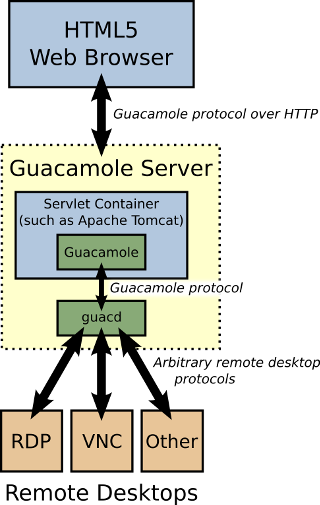
\includegraphics[scale=2]{main/images/guac-arch.png}
\end{center}
\caption{Architettura Guacamole.}
\label{fig:lifecycleComponent}
\end{figure}

La figura 4.1 mostra l'architettura di Guacamole. Si può notare in alto il client web per il monitoraggio delle connessioni e del loro stato. 

Il componente Guacd, all'interno del server, è il cuore di Guacamole che carica in modo dinamico il supporto per i protocolli desktop remoti (chiamati "plug-in client") e li collega ai desktop remoti in base alle istruzioni ricevute dall'applicazione web.
Guacd è un processo daemon che viene installato insieme a Guacamole e viene eseguito in background, ascoltando le connessioni TCP dall'applicazione Web. Guacd inoltre non comprende alcun protocollo specifico per desktop remoto, ma implementa abbastanza il protocollo Guacamole per determinare quale supporto di protocollo deve essere caricato e quali argomenti devono essere passati ad esso. Una volta caricato un plug-in client, viene eseguito indipendentemente da Guacd e ha il pieno controllo della comunicazione tra se stesso e l'applicazione Web fino al termine del plug-in client.

Guacamole è l'applicazione a cui si appoggia OVL Dashboard per instaurare le connessioni remote ai dispositivi. Esso mantiene le informazioni riguardanti utenti, permessi e dispositivi remoti in un database MySQL. Le funzionalità implementate in OVL Dashboard rendono possibile la completa gestione di queste informazioni, oltre a donare al sistema Guacamole un'interfaccia web più moderna e intuitiva.